\documentclass[]{standalone}

\usepackage{pgfplots}

\begin{document}

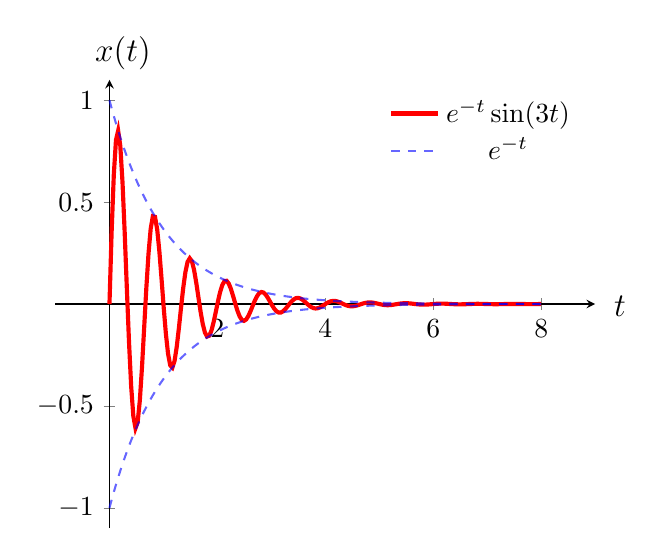
\begin{tikzpicture} 

	\begin{axis}
	[
	xlabel=$t$, ylabel=$x(t)$,
	axis lines = middle,
	>=latex,
	xmin = -1, xmax = 9, 
	ymin=-1.1, ymax=1.1,
	xlabel style={at={(1.075,0.45)}, font=\large},
	ylabel style={at={(0.125,1.0)},anchor=south, font=\large},
	legend style ={draw=none, fill=none, align=left},
	 ] 
	 
	 \addplot[domain=0:8, samples=200, line width=1.5pt, color=red]{exp(-x)*sin(deg(x*pi*3))};
	 
	 \addplot[domain=0:8, samples=200, line width=0.75pt, color=blue, opacity=0.6, dashed]{exp(-x)};
	 \addplot[domain=0:8, samples=200, line width=0.75pt, color=blue, opacity=0.6, dashed]{-exp(-x)};
	
	 \legend{$e^{-t} \sin(3t)$,$e^{-t}$, };
	
	\end{axis} 
	\end{tikzpicture}



\end{document}		  
